\documentclass[a4paper]{article}
\usepackage[english]{babel}
\usepackage{blindtext}
\usepackage{clrscode}
\usepackage{graphicx}
\usepackage{url}

\title{Q-learning for Fox and Hounds Board Game}
\author{Javad Bakhshi \and Martynas Budriunas}
\date{2012-05-29}

\begin{document}

\maketitle

\begin{abstract}
Q-learning is a popular machine learning technique for board games. In this
paper we present the application of it for a simple board game. It is different
from most of the other board games in that the players have different roles.
We have described a learning system design which can be implemented in a
memory-efficient way but still store all the data necessary for fast learning.
We also performed some experiments and provided our insights on the results,
from which one can easily find out that in this game the hounds are superior
than the fox.
\end{abstract}

\section{Introduction}
Fox and Hounds is a simple two-player board game. Traditionally it is played on
a chess board. One player controls the fox and the other controls four hounds.
Players have different goals. The fox has to reach the other side of the board,
and the hounds have to surround the fox so that it cannot move.

Initially the hounds are placed on all black squares in one row on the edge of
the board (Figure \ref{fig:board}). The fox can choose a starting position on
any of the black squares in the row on the opposite edge of the board. The
pieces can only move to unoccupied adjacent black squares. Additionally, the
hounds can only move forward. The players take alternative turns with the fox
moving first. On each turn only one of the hounds can be moved. The player who
cannot make a move loses.

\begin{figure}[htb]
\centering
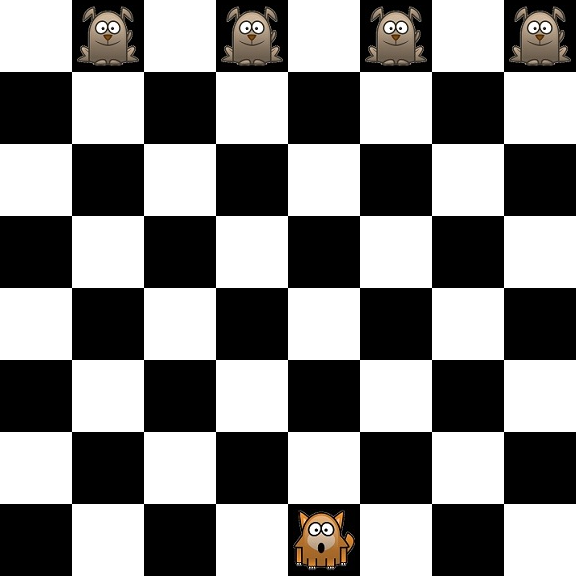
\includegraphics[width=0.6\textwidth]{board.png}
\caption{An example of initial board}
\label{fig:board}
\end{figure}

Fox and Hounds is an easy game aimed at young children. A human player can
easily find an optimal strategy for the hounds which guarantee victory (such a
strategy is described in \cite{berlekamp82}). In this project we try to
investigate how good a computer can be in finding that solution. To do that we
have implemented learning systems for both players based on Q-learning.

\section{Q-learning}
Q-learning is a reinforcement learning technique first presented in
\cite{watkins89}. Like in other reinforcement learning techniques, the agent is
presented with a state and can do one of several actions and the environment
responds by giving a reward. Using this technique each state-action pair $(s,
a)$ is assigned a Q-value $Q(s, a)$ which represents how much the agent favours
taking the action $a$ from a state $s$. In $\epsilon$-greedy Q-learning an agent
chooses a random action with probability $\epsilon$, and with probability $1 -
\epsilon$ it acts greedily -- performs an action with the highest Q-value.
After going to a state $s\prime$ and receiving a reward $r$, a Q-value is
updated using the following rule:
\[
    Q(s, a) \gets Q(s, a) + \eta [r + \gamma \max_{a\prime} Q(s\prime, a\prime)
    - Q(s, a)]
\]

Here and in the rest of the paper $\eta$ is a learning rate and $\gamma$ is a
discount factor. This way the agent is trained to seek higher sum of future
rewards.

Q-learning was applied to various board games. A very successful example is
TD\mbox{-}Gammon \cite{gerald95} -- a backgammon player which uses
temporal-difference learning, a generalization of Q-learning.

\section{Design}
In this game the players have different roles, so a separate learning system is
needed for both of them.

As shown in \cite{berlekamp82}, the hounds have a winning strategy, so to speed
up the learning we made the game slightly easier for the fox -- it wins as soon
as it reaches the same row as the last hound.

\subsection{States} \label{states}
Many games are troublesome to be solved by Q-learning because of a large number
of states. This game, however, has a number of states small enough to be stored
in a table. The number of states can be calculated as follows. There are 32
black squares on a board, and 4 of them are occupied by hounds. Since the
hounds do not differ, the number of their positions is $C_{32}^4 = \frac{32
\cdot 31 \cdot 30 \cdot 29}{4!} = 35960$. A fox can be in any of the remaining
28 black squares, so the total number of states is $35960 \cdot 28 + 1 =
1006881$. Here we added 1 because there is a special state when the fox is not
yet on the board (as mentioned in the introduction, in the beginning the fox
can choose any of the 4 squares in the row opposite from the hounds).

We have implemented the table as a two-dimensional array, where the index in
one dimension represents a state and in the other -- the action. The state is
encoded as an integer in range $[0, \frac{32!}{27! \cdot 4!}]$ as shown in the
following pseudocode.

\begin{codebox}
    \Procname{$\proc{StateToInt}(fox, hounds)$}
    \li \If $\proc{NotOnTheBoard}(fox)$
    \li     \Then \Return $32! / 28! / 4! \cdot 28$
        \End
    \li $state \gets 0$
    \li $foxCoordinate \gets 4 \cdot fox.row + fox.column$
    \li \For $i \gets 1$ \To 4 \>\>\>\>\> \Comment $hounds$ array is sorted in
                                                   ascending order of coordinate
    \li \Do $houndCoordinate \gets 4 \cdot hounds[i].row + hounds[i].column$
    \li     $state \gets state + C_{houndCoordinate}^i$
    \li     \If $fox.row > hounds[i].row$ \kw{or}
    \li \>\> $fox.row = hounds[i].row$ \kw{and} $fox.column > hounds[i].column$
    \li         \Then $foxCoordinate \gets foxCoordinate - 1$
            \End
        \End
    \li \Return $intState \cdot 28 + foxCoordinate$
    \End
\end{codebox}

The columns here are integers from 0 to 3 and the rows are integers from 0 to 7.
The coordinates are converted to integers by calculating $4 \cdot row +
column$. Arrangement of the hounds is one of 4-element subsets of a set of $8
\cdot 4 = 32$ elements. Lines 5--7 implement a method to enumerate those
combinations. It is based on a place of a subset in a lexicographic order of all
subsets $\{e_4, e_3, e_2, e_1\}$, $e_1 < e_2 < e_3 < e_4$. If $i$th hound has
a coordinate $e_i$, there are $C_{e_i}^i$ subsets for which elements to the
left from the $i$th are the same and the $i$th element is smaller than $e_i$
(for more details refer to \cite{knuth02}). Position of the fox is then
represented as a number from 0 to 27, which is an index of a square in a
sequence of empty squares left after placing the hounds, ordered by increasing
coordinate. This way the states are mapped to integers in the range $[0,
\frac{32!}{27! \cdot 4!})$ and the special case when the fox is not on the
board is encoded as $\frac{32!}{27!  \cdot 4!}$.

It can be proven that each state can only occur after a move of a certain
player. Notice that the sum of the rows of all pieces modulo 2 is an invariant
with value 0 before fox's move and 1 before hounds' move. This means that the
number of states for one learning system's table of Q-values can be a half of
the total number of states.

\subsection{Actions}
Each fox can do at most 4 actions. In the initial state when it is not on the
board yet, it can choose any of the 4 black squares in the row on the side of
the board opposite from the hounds. Note that this is the only case when a fox
moves twice in a row, as it begins the game. From all the other states the fox
can move to any of the unoccupied adjacent squares, of which there are at most
4.

The hounds can do at most 8 actions -- each of the 4 hounds can move in up to 2
directions.

\section{Experiments}
To run an experiment we repeat the following two phases:
\begin{enumerate}
    \item {\em Training phase.} Let the training systems play against each other for
        100,000 turns.
    \item {\em Evaluation phase.} Set learning rates to 0. Set the exploration
        rate of one system to 0, play 100 games and record the number of wins
        of the other system. Then do the same evaluation of the other learning
        system. Reset the learning rates and exploration rates to the initial
        values afterwards for the next training phase.
\end{enumerate}

Note that we cannot evaluate both learning systems at the same time by setting
their exploration rates to zero, because then all the games are likely to be
the same (there would be some variation only if a player reaches the state from
which there are several actions with the same maximum Q-value). Because of that
the sum of wins of both players in one evaluation is not necessary (and rarely
is) 100.

The exact algorithms and scenarios of running the following experiments can be
found in our source code repository \cite{github}.

\subsection{Experiment 1}
To begin we present the results of an experiment of both fox and hounds playing
randomly (all parameters are 0). Clearly the fox has an advantage in this
situation.

\input{exp1.tex}

\subsection{Experiment 2}
In this experiment we wanted to find out the best parameters for training the
hounds against randomly playing fox.

\input{exp2graph1.tex}

\input{exp2graph2.tex}

From the many learning rates we have tried, 0.5 seems to produce the fastest
learning, as can be observed by comparing the two graphs above. Higher
discount factor resulted in a better stability in the long run. The instances
with $0.2$ exploration rate reached very high evaluation scores a couple
million turns earlier than the ones with $\epsilon = 0.1$.

\subsection{Experiment 3}
This time we trained the foxes the same way as in experiment 2 we trained the
hounds.

\input{exp3graph1.tex}

\input{exp3graph2.tex}

Since even the random foxes performed very well against random hounds
(Experiment 1), it is no surprise that it did not take long for them to learn
to almost never lose in this experiment.

\subsection{Experiment 4}
In this experiment we further train first two hounds from experiment 2 against
first two foxes from experiment 3.

\input{exp4graph1.tex}

\input{exp4graph2.tex}

\input{exp4graph3.tex}

\input{exp4graph4.tex}

As we can see the hounds trained in experiment 2 lose seldom. Foxes are also
well-trained and can often take advantage of even such a well-trained hounds'
exploration. In the cases where hounds' exploration was higher, foxes performed
better.

\subsection{Experiment 5}
We further examine the performance of both players learning from scratch.

\input{exp5graph1.tex}

\input{exp5graph2.tex}

\input{exp5graph3.tex}

\input{exp5graph4.tex}

We can clearly see that the hounds reliably learn the right strategy, as their
performance improves from the very low in the begining to the very high in the
end. The fox has no other choices than to learn taking advantage of suboptimal
hounds' turns when they explore. However, as we can see, the foxes are doing it
well and even a small exploration of hounds can let the fox win most of the
times.

The following graph compares the number of states visited by the players with
exploration rate 0.1 (Graph 1) and 0.2 (Graph 4).

\input{exp5graph5.tex}

The total number of states for one player is more than 400 thousand. From this
graph we can see why the hounds still occationally lose in our experiments, as
they have not yet explored all of the states. But even having explored less
than a half of the states they steadily win more than 99\% of times on average.

\section{Conclusions and Future Work}
We have found out that Q-learning is a suitable technique for machine learning
systems that play Fox and Hounds. Contrary to many other games played on a chess
board, the states of this game can be expressed in a range of integers which is
small enuogh to store all the Q-values in a table. Because of that the learning
system does not have to depend on other learning systems for storing that data
and can learn fast. The results of our experiments also conform with the fact
that the hounds have a winning strategy as proved in \cite{berlekamp82}, and we
could derive it from the table of Q-values of a trained player.

Our learning system design can be further improved by reducing the Q-values
table size by a factor of 2, as proposed in section \ref{states}. Another
improvement of a learning system could be a dynamic adjustment of the
parameters based on the results (for example, decrease the exploration if the
learning system is doing well, and increase it otherwise). We have already
produced all the tools needed to run such experiments, which can be found at
our source code repository \cite{github}.

\begin{thebibliography}{9}
\bibitem{watkins89}
    Chris Watkins,
    {\em Learning from Delayed Rewards}.
    PhD Thesis, University of Cambridge, 1989.
\bibitem{gerald95}
    Gerald Tesauro,
    {\em Temporal difference learning and TD-Gammon}.
    Communications of the ACM,
    Volume 38 Issue 3, March 1995.
\bibitem{berlekamp82}
    E. Berlekamp, J. Conway, R. Guy,
    {\em Winning Ways for your Mathematical Plays}.
    Volume 2, 1982, pp. 635--645.
\bibitem{knuth02}
    Donald E. Knuth,
    {\em Generating All Combinations and Partitions}.
    The Art of Computer Programming, Volume 4, Fascicle 3, Addison-Wesley, pp.
    5-−6.
\bibitem{github}
    \url{https://github.com/mabu/Fox-and-Hounds}
\end{thebibliography}

\end{document}

